% Kapitel 1
% Die Unterkapitel können auch in separaten Dateien stehen,
% die dann mit dem \include-Befehl eingebunden werden.
%-------------------------------------------------------------------------------

\chapter{Einleitung}
Die Datenbank WiReLib repräsentiert die den Bestand der Bibliothek für das Institut für Wissenschaftliches Rechnen.
Auf diese Datenbank können Nutzer über ein Web-Interface zugreifen um Dokumente zu suchen und sich nach der Anmeldung Dokumente auszuleihen.

\section{Projektdetails}
Die Funktionalitäten gliedern sich in drei Teilbereiche.
Diese Bereiche bündeln die Anforderungen, die im Pflichtenheft spezialisiert
worden sind.

\begin{figure}[h]
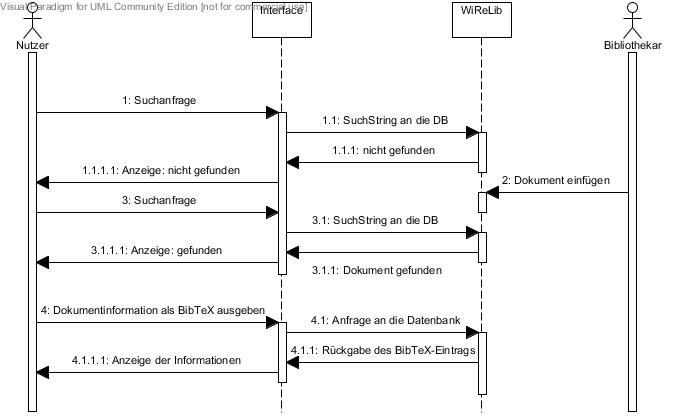
\includegraphics[width=0.8\linewidth]{bilder/sequenz-uebersicht.jpg}
\caption[Sequenzdiagramm-Übersicht]{Sequenzdiagramm-Übersicht}
\label{Sequenzdiagramm-Übersicht}
\end{figure}

\subsection{Client}
Über das Web-Interface erhält der als Client fungierende Browser Zugriff auf die Datenbank und kann verschiedene Funktionen nutzen.

\subsection{Server}
Auf dem Server läuft die Anwendung, welche verschiedene Funktionen zum Auslesen und Verwalten der Datenbank bereitstellt. 
Auch stellt der Server die Datenbank bereit und baut eine sichere Verbindung zum Client auf.

\subsection{Datenbank}
In der Datenbank werden die Dokumenente sowie die Nutzerrechte verwaltet.
Auch werden Daten zu den einzelnen Nutzern gespeichert um diese zu identifizieren und im Falle des Ablaufs der Verleihfrist zu benachrichtigen.
